% ============================================================
%  chapter11_aixi_mdp_slides.tex
%  Chapter 11: AIXI-MDP
%  An Introduction to Universal Artificial Intelligence
%  Hutter, Quarel & Catt --- CRC Press, 2024
% ============================================================
\documentclass[aspectratio=169,10pt]{beamer}

\usetheme{Madrid}
\usecolortheme{seahorse}
\usefonttheme{professionalfonts}

% -- packages ------------------------------------------------------------------
\usepackage{amsmath,amssymb,bm}
\usepackage{graphicx}
\usepackage{booktabs}
\usepackage{listings}
\usepackage{xcolor}
\usepackage{tikz}
\usetikzlibrary{shapes,arrows,positioning,calc}
\usepackage{mathtools}
\usepackage{array}
\usepackage{multirow}
\usepackage{makecell}
\usepackage{stmaryrd}

\graphicspath{{figures/}}

% -- listings style --------------------------------------------------------
\lstdefinestyle{pythonstyle}{
  language=Python,
  basicstyle=\ttfamily\scriptsize,
  keywordstyle=\color{blue}\bfseries,
  stringstyle=\color{orange},
  commentstyle=\color{green!50!black}\itshape,
  numberstyle=\tiny\color{gray},
  numbers=left,
  stepnumber=1,
  numbersep=5pt,
  frame=single,
  backgroundcolor=\color{gray!7},
  breaklines=true,
  showstringspaces=false,
  tabsize=2,
  captionpos=b,
}
\lstset{style=pythonstyle}

% -- beamer setup -----------------------------------------------------------
\setbeamertemplate{footline}[frame number]
\setbeamertemplate{navigation symbols}{}
\setbeamersize{text margin left=0.5cm, text margin right=0.5cm}

% -- convenient macros -------------------------------------------------------
\newcommand{\explain}[1]{\par\smallskip{\footnotesize\itshape #1}\par}
\newcommand{\Mmdp}{\mathcal{M}_{\mathrm{MDP}}}
\newcommand{\ximdp}{\xi_{\mathrm{MDP}}}
\newcommand{\Rmat}{\mathfrak{R}}
\newcommand{\Acal}{\mathcal{A}}
\newcommand{\Ocal}{\mathcal{O}}
\newcommand{\hlt}{h_{<t}}

% -- title -------------------------------------------------------------------
\title[UAI -- Ch.11 AIXI-MDP]{An Introduction to Universal Artificial Intelligence}
\subtitle{Chapter 11: AIXI-MDP}
\author{Based on Hutter, Quarel \& Catt}
\institute{CRC Press, 2024}
\date{}

% =============================================================================
\begin{document}
% =============================================================================

\begin{frame}
  \titlepage
  \begin{center}
  \small\itshape ``Simplicity is the ultimate sophistication.'' --- Leonardo da Vinci
  \end{center}
\end{frame}

\begin{frame}{Outline}
  \tableofcontents
\end{frame}

% =============================================================================
\section{11.1 AIXI-MDP Setup}
% =============================================================================

\begin{frame}[allowframebreaks]{From AIXI to a Computable Approximation}
  \textbf{Where we are.} Earlier chapters introduced universal (Bayesian)
  models of prediction (sequence prediction, CTW) and decision-making
  (the general history-based agent AI$\xi$ ($\xi$ is pronounced ``xi''), and
  its universal instantiation AIXI). AIXI served as a \emph{gold standard}:
  a mathematically well-defined, maximally intelligent agent that we can use
  to judge other agents, even though AIXI itself is not something we can run
  on a computer.

  \bigskip
  \textbf{Why AIXI cannot be run directly.} Two obstacles stand in the way:
  \begin{itemize}
    \item The Kolmogorov complexity $K(x)$ (the length of the shortest
      program that outputs the string $x$ -- a measure of how ``simple'' or
      ``compressible'' $x$ is) is \textbf{incomputable}: no algorithm can
      calculate it in general. Since the Solomonoff mixture
      $M=\xi_U$ is built out of $K(x)$, it is incomputable too.
    \item Even if we could evaluate the mixture, the \textbf{expectimax}
      search (alternating maximization over actions and expectation over
      observations, all the way to the planning horizon) that AIXI performs
      is computationally intractable for essentially any real problem: its
      cost explodes exponentially with the horizon.
    \end{itemize}
  \explain{$K(x)$ is Kolmogorov complexity: the length, in bits, of the
  shortest computer program that prints the string $x$ and then stops. It is
  a rigorous notion of ``simplicity,'' but famously cannot be computed by
  any algorithm. $M=\xi_U$ is the Solomonoff mixture: a weighted average
  over all computable environments, weighting simpler (lower-$K$)
  environments more heavily -- it is the ideal universal predictor, but
  inherits $K(x)$'s incomputability.}

  \framebreak

  \textbf{The plan for this part of the book.} Since we cannot use AIXI
  as-is, we build \emph{systematic computable approximations} of it:
  \begin{itemize}
    \item \textbf{This chapter (11):} the first and simplest instantiation
      of AI$\xi$, called \textbf{AIXI-MDP}, where $\xi$ is a very efficiently
      computable mixture over \textbf{Markov Decision Processes (MDPs)}. An
      MDP is a simple kind of environment whose next observation depends
      only on the most recent action and observation, not the full history.
    \item \textbf{Chapter 12:} a more advanced, more broadly applicable
      instantiation of AI$\xi$.
    \item \textbf{Chapter 13:} some further approximations that are
      powerful in theory but not yet practical.
  \end{itemize}

  \bigskip
  \textbf{This chapter's testbed.} We run AIXI-MDP on the classic repeated
  $2\times2$ matrix games from Section 10.2: \emph{Prisoner's Dilemma},
  \emph{Stag Hunt}, \emph{Chicken}, \emph{Battle of the Sexes}, and
  \emph{Matching Pennies}. Because the action and observation spaces here
  are just $\{0,1\}$ (one bit each), the action/perception spaces are small
  enough that we can \textbf{brute-force compute} the Bayes-optimal policy
  $\pi_\xi^*$ directly from the expectimax expression (Theorem 7.4.2), with
  no further approximation needed beyond restricting $\xi$ to MDPs.
\end{frame}

% -----------------------------------------------------------------------------
\begin{frame}[allowframebreaks]{Emulating Simultaneous Actions}
  Repeated matrix games are usually \emph{simultaneous}: both players choose
  their action at the same time, each ignorant of what the other just chose.
  AIXI, however, was described using the usual \textbf{cybernetic model} for
  reinforcement learning, in which there is a strict order: the agent acts,
  the environment receives that action, and only afterwards does the
  environment send back a \emph{percept} (an observation-reward pair). These
  two pictures seem incompatible -- but we can reconcile them with a small
  trick.

  \bigskip
  \textbf{The trick.} We hide the opponent \emph{inside} the environment,
  and we constrain the type of distribution the opponent (as part of the
  environment) is allowed to use: the opponent's policy is not allowed to
  depend on the agent's most recently issued action. This exactly captures
  ``the opponent did not see what I just did.''

  \framebreak

  \textbf{One iteration of the interaction loop:}
  \begin{itemize}
    \item The agent takes action $a_t$, but the environment does not yet
      receive it.
    \item The opponent (who is part of the environment) takes action
      $a_t'$, ignorant of the agent's choice of $a_t$.
    \item The environment receives \emph{both} actions $a_t$ and $a_t'$,
      and then, using the \textbf{reward matrix} $\Rmat$ ($\Rmat$ is a
      capital Fraktur R -- the pay-off matrix from game theory, Section
      10.2.2), computes the reward $r_t$ for the agent (taking $a_t$ against
      opponent action $a_t'$) and the reward $r_t'$ for the opponent
      (taking $a_t'$ against agent action $a_t$).
    \item The agent receives reward $r_t$ and observation $o_t=a_t'$. The
      opponent receives reward $r_t'$ and observation $o_t'=a_t$. In other
      words: each player is told the reward matrix entry they earned, plus,
      as extra side information, the other player's most recently played
      action.
    \item The time step increments, $t:=t+1$, and we loop.
  \end{itemize}

  \begin{center}
    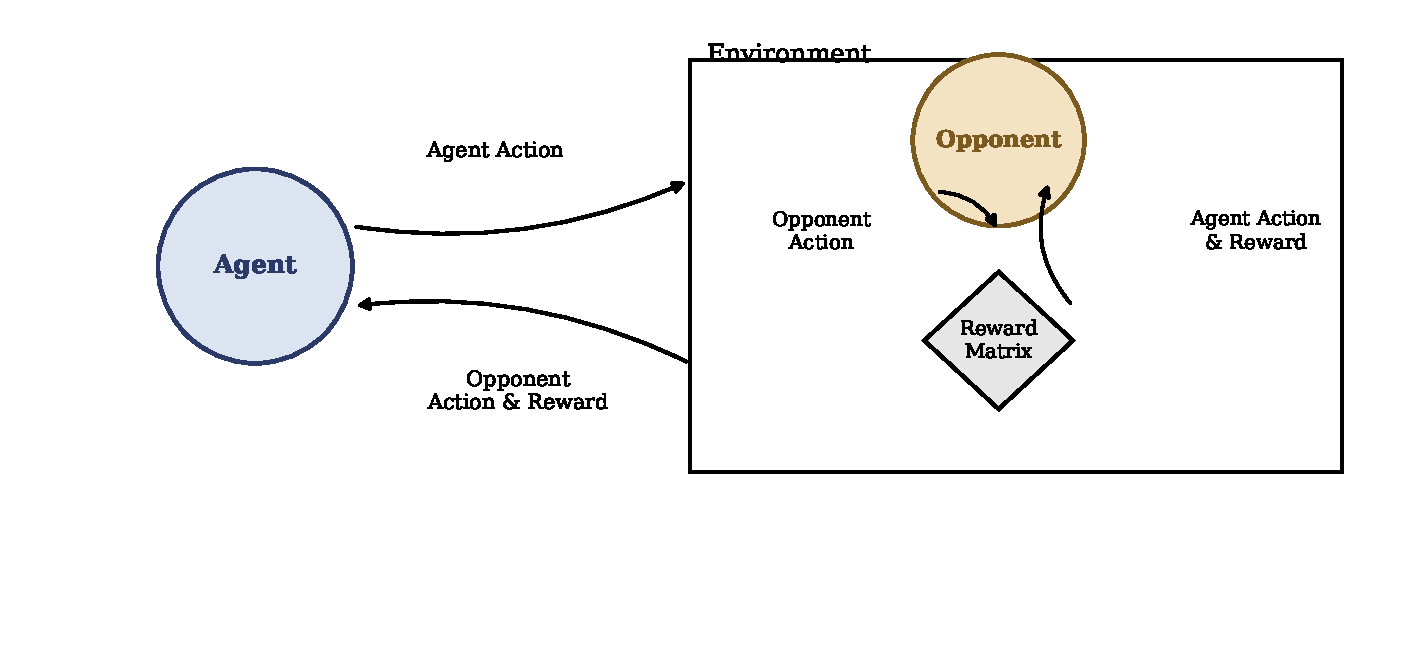
\includegraphics[width=0.72\textwidth]{fig11_1_interaction_loop}
  \end{center}
  {\footnotesize \textbf{Figure 11.1.} How repeated normal-form games with
  simultaneous actions are realized within the usual cybernetic (act-then-
  perceive) model, by hiding the opponent inside the environment and
  withholding the most recent action from it.}

  \framebreak

  \textbf{Environment-agent (a)symmetry.} The environment is \emph{not} the
  same thing as the opponent: the environment also includes the reward
  matrix and manages the whole interaction loop. From the agent's point of
  view, the opponent is just one part of a larger environment. Symmetrically,
  we could redraw Figure 11.1 from the opponent's perspective, in which case
  the opponent would view the reward matrix, the interaction loop,
  \emph{and} the agent together as its own ``environment.''

  \bigskip
  \textbf{Implicit knowledge.} Both players are implicitly aware of the
  other's most recently received reward as well ($r'_{t-1}$ for the agent,
  $r_{t-1}$ for the opponent), since both players know the full reward
  matrix $\Rmat$ and each other's last action. This lets us simplify
  notation: we can write the agent's observation as $o_t=a_t'$ (just the
  opponent's action) rather than the pair $o_t=(a_t',r_t')$, without losing
  any information, because $r_t'$ is fully determined by $(a_t,a_t')$ and
  $\Rmat$.
\end{frame}

% -----------------------------------------------------------------------------
\begin{frame}[allowframebreaks]{Known Reward Matrix and a Markov Opponent}
  \textbf{Withholding the last action from the history.} Since in this
  chapter the agent is told the reward matrix $\Rmat$ in advance, the reward
  $r_t=\Rmat(a_t,o_t)$ is just a known deterministic function of the action
  $a_t$ and observation $o_t$ -- so we can safely drop $r_t$ from the
  history and only track the \emph{observation-action} history
  $$\hlt := (oa)_{<t} = o_1a_1 \ldots o_{t-1}a_{t-1}.$$
  \explain{$\hlt$ (read: ``h sub less-than $t$'') denotes everything the
  agent has seen and done before time $t$. Notice the order: observation
  \emph{then} action within each round, because $o_t$ depends on the
  previous observation and action, but never on the agent's \emph{current}
  action $a_t$ -- this is exactly the ``opponent can't see what I just did''
  property we built into the loop above.}
  \bigskip

  A footnote in the book flags that Chapter 12 will relax this: there, the
  agent is \emph{not} told the reward matrix or even the rules of the game
  in advance, and must learn those too.

  \framebreak

  \textbf{Markov environments.} The agent additionally \emph{assumes} that
  the environment (and hence the opponent inside it) is a
  \textbf{Markov Decision Process (MDP)}: the next observation only depends
  on the single most recent action-observation pair, not on the entire
  history. Formally, if $\mu$ ($\mu$ is pronounced ``mu'' and denotes the
  true environment) is Markov, then
  $$\mu(o_t \mid \hlt) = \mu(o_t \mid o_{t-1}a_{t-1}).$$
  \explain{This says: to predict the next observation $o_t$, you only need
  to remember the very last observation-action pair $(o_{t-1},a_{t-1})$ --
  everything further back in the history is irrelevant. This is what
  ``Markov'' means: no long-term memory is needed.}

  \bigskip
  Even though the \emph{environment} is assumed Markov, the \emph{agent
  itself} remains history-based: it still conditions its action choice on
  the entire interaction history $\hlt$, hoping to detect and exploit
  statistical regularities in how the opponent responds.

  \framebreak

  \textbf{No Grain of Truth.} These two assumptions -- known reward matrix,
  Markov opponent -- can cause trouble. Consider AIXI-MDP playing against a
  copy of itself. Neither agent can learn that its opponent is
  \emph{also} another instance of AIXI-MDP; instead, each concentrates its
  posterior belief $\xi$ on whichever model $\nu\in\mathcal M$ ($\nu$ is
  pronounced ``nu'' and denotes a candidate environment model; $\mathcal M$
  is the model class, i.e., the whole collection of models the agent
  entertains) best fits the observations so far. In other words, the class
  $\Mmdp$ of Markov models does \textbf{not} contain a \emph{Grain of
  Truth} (recall Section 10.6: a model class ``has a Grain of Truth'' if the
  true environment, or something behaviourally equivalent to it, is actually
  inside the class).

  \bigskip
  \textbf{This is a deep, general problem, not just an MDP quirk:} even
  playing a true copy of AIXI against itself, using the richer model class
  $\mathcal M_{sol}$ of \emph{all} computable environments, runs into the
  same issue -- AIXI is not contained in its own model class, because AIXI
  itself is non-computable! The only known model class with a genuine Grain
  of Truth is the class of \textbf{Reflective Oracle} machines
  $\mathcal M_r^O \supset \mathcal M_{comp}$ (Theorem 10.6.2), which we will
  not need for AIXI-MDP.
\end{frame}

% -----------------------------------------------------------------------------
\begin{frame}{Binary Action and Observation Space}
  This whole setup is general -- it works for any class of games with any
  number of actions or opponents. In this chapter we specialize to the
  simplest interesting case:

  \begin{block}{The $2\times2$ matrix-game setting of this chapter}
    \begin{itemize}
      \item A single opponent, and repeated $2\times2$ matrix games.
      \item Both the action space and the observation space are binary:
        $\Acal=\Ocal=\{0,1\}$ ($\Acal,\Ocal$ are the sets of possible
        actions/observations -- ``script A,'' ``script O'').
      \item The observation $o_t$ is exactly the action the opponent chose
        on the previous round.
      \item In each game the agent and opponent are given a reward matrix
        $\Rmat$, giving the reward for each observation-action pair
        $(o,a)$.
      \item The agent additionally has access to the full history $\hlt$,
        which records every action taken and every observation received by
        both players so far (implicitly -- see the previous frame).
    \end{itemize}
  \end{block}
  \explain{A ``$2\times2$ matrix game'' just means: there are 2 players,
  each with 2 possible actions (say, ``cooperate''/``defect'' or
  ``swerve''/``go straight''), and the reward for each combination of the
  two players' choices is listed in a $2\times2$ table -- the reward matrix
  $\Rmat$. This is exactly the classical setting used for games like
  Prisoner's Dilemma, discussed in Section 10.2.3 and revisited in Section
  11.3 below.}
\end{frame}

% -----------------------------------------------------------------------------
\begin{frame}[fragile]{Python: One Round of the Interaction Loop}
  A concrete, tiny example of the loop from Figure 11.1, using the classic
  Prisoner's Dilemma reward matrix (action/observation $0=$``cooperate'',
  $1=$``defect''): mutual cooperation pays 3, mutual defection pays 1, and
  defecting against a cooperator pays 5 (with the sucker getting 0.)
  \begin{lstlisting}[language=Python]
# Reward matrix R[a][o]: reward to the agent for action a
# against opponent action (=observation) o.
R = {(0, 0): 3, (0, 1): 0,   # agent cooperates: 3 if opp. cooperates, 0 if opp. defects
     (1, 0): 5, (1, 1): 1}   # agent defects:    5 if opp. cooperates, 1 if opp. defects

def one_round(a_t, a_opp):
    """One iteration of Figure 11.1's loop (rewards computed simultaneously)."""
    r_t   = R[(a_t, a_opp)]        # agent's reward
    r_opp = R[(a_opp, a_t)]        # opponent's reward (R read with roles swapped)
    o_t, o_opp = a_opp, a_t        # each side observes the other's action
    return r_t, o_t, r_opp, o_opp

# Agent defects (1), opponent (e.g. "tit-for-tat") cooperates (0) this round:
r_t, o_t, r_opp, o_opp = one_round(a_t=1, a_opp=0)
print(f"agent reward={r_t}, agent obs={o_t} | opp reward={r_opp}, opp obs={o_opp}")
# -> agent reward=5, agent obs=0 | opp reward=0, opp obs=1
  \end{lstlisting}
  \explain{The agent defects while the opponent cooperates, so the agent
  gets the ``temptation'' reward of 5 and observes that the opponent
  cooperated ($o_t=0$); the opponent gets the ``sucker'' reward of 0 and
  observes that the agent defected ($o_{opp}=1$).}
\end{frame}

% =============================================================================
\section{11.2 Definition of AIXI-MDP}
% =============================================================================

\begin{frame}[allowframebreaks]{Recursive Q-Value Function of AIXI-MDP}
  \textbf{Definition.} AIXI-MDP is simply AI$\xi$ (recall: the general
  Bayesian agent) with the model class $\mathcal M$ set to $\Mmdp$, the
  class of Markov Decision Processes over $\Acal\times\Ocal$, described
  below. Any of the three equivalent characterizations of AI$\nu$ from
  Chapter 6 can be adapted here: the abstract expectation-policy forms
  (Definitions 6.6.1, 6.7.1), the explicit iterative form (Lemma 6.6.3), or
  the (pseudo)recursive Bellman form (Theorem 6.7.2). We use the last one,
  with $\nu=\xi$.

  \bigskip
  In strategic game theory it is common to \emph{neither discount nor
  normalize} rewards. Plugging this choice ($\gamma_t=1=\Gamma_t$;
  $\gamma$ is ``gamma,'' the discount factor, and $\Gamma_t$ its running
  normalizer) into the general Bellman optimality equation (6.7.3)/(6.7.5)
  for the optimal policy $\pi_\xi^*$ gives
  $$Q_\xi^{*,m}(\hlt,a_t) = \sum_{e_t}\xi(e_t\mid \hlt a_t)\Bigl[r_t +
  \max_{a_{t+1}}Q_\xi^{*,m}(h_{1:t},a_{t+1})\Bigr]$$
  with history $h_{1:t}:=a_1o_1r_1\ldots a_to_tr_t$.
  \explain{$Q^{*,m}_\xi(\hlt,a_t)$ is the \emph{optimal Q-value}: the best
  total reward the agent can expect to collect from now (time $t$) up to
  the planning horizon $m$, if it takes action $a_t$ right now and then
  plays optimally afterwards, given everything it has seen ($\hlt$) and
  believing the mixture $\xi$. The sum is over $e_t=(o_t,r_t)$, all
  possible percepts (observation+reward pairs) the environment could send
  back; $\xi(e_t\mid\hlt a_t)$ is how likely $\xi$ thinks each one is.}

  \framebreak

  \textbf{Simplifying for known, deterministic rewards.} Now
  $r_t=\Rmat(a_t,o_t)$ is a known deterministic function of $a_t$ and
  $o_t$, so we can drop $r_t$ from the history entirely, and the percept
  $e_t=o_tr_t$ becomes just $o_t$. Moreover, since the environment (the
  opponent) never sees the agent's current action $a_t$ before choosing its
  own action $a_t'=o_t$, we only need to consider models $\nu\in\mathcal M$
  for which $\nu(e_t\mid\hlt a_t)$ -- and hence $\xi(e_t\mid\hlt a_t)$ --
  does not actually depend on $a_t$. Putting this together:

  \begin{block}{Equation (11.2.1) --- AIXI-MDP's recursive Q-value}
    $$Q_\xi^{*,m}(\hlt,a_t) = \sum_{o_t}\xi(o_t\mid\hlt)
    \Bigl[\Rmat(a_t,o_t) + \max_{a_{t+1}}Q_\xi^{*,m}(h_{1:t},a_{t+1})\Bigr]$$
  \end{block}
  \explain{Plain English: to value taking action $a_t$ now, weigh each
  possible opponent response $o_t$ by how likely $\xi$ thinks it is,
  add the immediate reward $\Rmat(a_t,o_t)$ that response would earn, plus
  the best value achievable from then on (the $\max_{a_{t+1}}$ term,
  computed the same way one step deeper) -- and sum it all up. The
  recursion \textbf{terminates} once $t$ exceeds the horizon $m$, where we
  set $Q=0$ (there is no more future to plan for).}
\end{frame}

% -----------------------------------------------------------------------------
\begin{frame}[allowframebreaks]{The MDP Model Class and the Mixture $\ximdp$}
  \textbf{Computing $\ximdp$.} The agent assumes the environment is Markov
  and cannot see its own last action, i.e.\ $\mu(e_t\mid\hlt a_t) =
  \mu(o_t\mid o_{t-1}a_{t-1})$. $\Mmdp$ is the class of \emph{all}
  environments $\nu$ satisfying this property, and $\ximdp$ is a
  \textbf{Bayesian mixture} over $\Mmdp$ with a prior $w$ specified below.
  \explain{A Bayesian mixture is a weighted blend of many candidate models,
  where models that fit the data seen so far get more weight over time.
  Here the candidate models are all possible Markov transition rules over
  the binary action/observation space, and $\ximdp$ is the specific blended
  predictor built from them.}

  \bigskip
  Every Markov environment over $\Acal=\Ocal=\{0,1\}$ can be encoded as a
  vector $(\theta_{00},\theta_{01},\theta_{10},\theta_{11})\in[0,1]^4$
  ($\theta$ is pronounced ``theta''), one number $\theta_{ao}$ for each of
  the 4 possible most-recent action-observation pairs
  $(o_{t-1},a_{t-1})\in\{(0,0),(0,1),(1,0),(1,1)\}$, giving the probability
  that the opponent produces observation $o_t=0$ given that pair.

  \framebreak

  \textbf{The prior.} For the mixture, we assume each $\theta_{ao}$ is
  independently and uniformly distributed, $\theta_{ao}\sim\mathcal
  U([0,1])$, i.e.\ following the \emph{principle of indifference} (all
  values in $[0,1]$ equally likely a priori): prior density
  $w(\theta)=1$ for $\theta\in[0,1]^4$.

  \bigskip
  \textbf{Counting statistics.} Let $n_{ao}^t$ be the number of times the
  action-observation pair $ao$ has appeared in $\hlt$, and let
  $n_{ao\cdot o'}^t$ be the number of those times that were \emph{followed}
  by the next observation $o'$. The dot ``$\cdot$'' just means ``we don't
  care what action came next,'' since the environment is independent of it.
  Formally,
  $$n_{ao}^t := \bigl|\{\tau<t : a_\tau=a \wedge o_\tau=o\}\bigr|, \qquad
  n_{ao\cdot o'}^t := \bigl|\{\tau<t : a_\tau=a \wedge o_\tau=o \wedge
  o_{\tau+1}=o'\}\bigr|.$$
  \explain{$\tau$ (pronounced ``tau'') is just a dummy index running over
  past time steps. $n_{ao}^t$ counts how many times, somewhere in the
  history so far, the pair (action $a$, observation $o$) occurred and was
  itself followed by another recorded observation; $n_{ao\cdot o'}^t$
  additionally requires that following observation to equal $o'$. These are
  exactly the ``successes'' and ``trials'' we need for a Bernoulli
  (coin-flip-like) estimate of $\theta_{ao}$.}

  \framebreak

  This 1st-order Markov process was already studied in Section 4.2.1. The
  sub-process of just the $o_{t+1}$'s that follow $a_to_t=ao$ is a
  \textbf{Bernoulli$(\theta_{ao})$ process} ($\theta_{ao}$ being the unknown
  success probability). Bayes-mixing it with a uniform prior over
  $\theta_{ao}$ gives the familiar \textbf{Laplace estimator}, derived
  earlier in Section 2.4.3. In our notation:

  \begin{block}{Equation (11.2.2) --- The MDP estimator $\ximdp$ (Laplace rule)}
    $$\ximdp(o_t\mid\hlt) = \frac{n^t_{a_{t-1}o_{t-1}\cdot o_t}+1}
    {n^t_{a_{t-1}o_{t-1}}+2}$$
  \end{block}
  \explain{To predict the next observation $o_t$, look only at the
  \emph{most recent} action-observation pair $(a_{t-1},o_{t-1})$ (Markov
  assumption), count how many times in the past that exact pair was
  followed by $o_t$ (numerator, plus a pseudo-count of $1$), and divide by
  how many times that pair occurred at all (denominator, plus a
  pseudo-count of $2$ -- one for each possible outcome $o_t\in\{0,1\}$).
  This ``add-one'' correction is exactly Laplace's rule of succession: with
  zero data it defaults sensibly to probability $\tfrac12$, and it never
  outputs exactly $0$ or $1$.}

  \bigskip
  Note $\ximdp\notin\Mmdp$: unlike any single $\nu\in\Mmdp$, $\ximdp$
  itself depends on the \emph{whole} history (through the counts), not just
  the last pair -- computing $\ximdp$ has been reduced to counting
  occurrences of a substring in a string, which is cheap: $O(1)$ time per
  $t$, done incrementally.

  \bigskip
  \textbf{Comparison to the KT estimator} (Definition 4.1.1): the KT
  estimator uses a slightly different (Jeffreys) prior (Definition 2.4.11),
  which \emph{halves} the $1$ and $2$ appearing in the Laplace rule:
  $\ximdp^{KT}(o_t\mid\hlt) = \dfrac{n^t_{a_{t-1}o_{t-1}\cdot o_t}+0.5}
  {n^t_{a_{t-1}o_{t-1}}+1}$. Both are simple, regularized frequency
  estimators.
\end{frame}

% -----------------------------------------------------------------------------
\begin{frame}[fragile]{Python: Laplace vs.\ KT Estimator, By Hand}
  Suppose the pair (action $=1$, observation $=1$) has occurred $n=5$ times
  in the history so far, and the observation that followed it was, in
  order, $1,0,1,1,0$ (so $3$ of the $5$ were followed by a $1$). Running
  estimates after each new data point:
  \begin{lstlisting}[language=Python]
followups = [1, 0, 1, 1, 0]     # o' observed after each occurrence of pair (a=1,o=1)
n, n1 = 0, 0
print(f"{'n':>2} {'n1':>3}  {'Laplace (n1+1)/(n+2)':>22}  {'KT (n1+0.5)/(n+1)':>18}")
for outcome in followups:
    n += 1
    n1 += outcome
    laplace = (n1 + 1) / (n + 2)
    kt      = (n1 + 0.5) / (n + 1)
    print(f"{n:>2} {n1:>3}  {laplace:>22.4f}  {kt:>18.4f}")
  \end{lstlisting}
  {\scriptsize
  \begin{verbatim}
   n  n1     Laplace (n1+1)/(n+2)    KT (n1+0.5)/(n+1)
   1   1                  0.6667                0.7500
   2   1                  0.5000                0.5000
   3   2                  0.6000                0.6250
   4   3                  0.6667                0.7000
   5   3                  0.5714                0.5833
  \end{verbatim}}
  \explain{Both estimators track the empirical frequency $n_1/n$ closely
  but pull it slightly toward $0.5$, especially when $n$ is small (compare
  row $n=1$: raw frequency would say $1.0$, but Laplace says only
  $0.667$ and KT $0.75$). This is exactly the regularizing effect of the
  Bayesian prior.}
\end{frame}

% -----------------------------------------------------------------------------
\begin{frame}[allowframebreaks]{Algorithm 11.1: Computing $Q^{*,m}_{\ximdp}$}
  We now have everything needed to compute $Q^{*,m}_{\ximdp}(\hlt,a_t)$ via
  (11.2.1). Algorithm 11.1 spells out this recursion explicitly for the
  special case of binary action and observation spaces relevant to
  $2\times2$ matrix games (the general case, for any $|\Acal\times\Ocal|$,
  is essentially the same).

  \begin{block}{Algorithm 11.1 (Q-value function of AIXI-MDP $Q^{*,m}_{\ximdp}(\hlt,a_t)$)}
  \textbf{Require:} horizon $m$; MDP estimator $\ximdp$ (Eq.~11.2.2); reward
  matrix $\Rmat\in\mathbb R^{2\times2}$. \\
  \textbf{Input:} history $\hlt$, action $a_t$. \\
  \textbf{Output:} Q-value $Q^{*,m}_{\ximdp}(\hlt,a_t)$.
  \begin{enumerate}
    \item \textbf{if} $m<t$ \textbf{then return} $0$
    \item \textbf{return}\ \ $\ximdp(0\mid\hlt)\cdot\bigl[\Rmat(a_t,0) +
      \max\{Q^{*,m}_{\ximdp}(\hlt a_t 0,0),\, Q^{*,m}_{\ximdp}(\hlt a_t0,1)\}\bigr]$
    \item[] \hspace{1.7em}$+\ \ximdp(1\mid\hlt)\cdot\bigl[\Rmat(a_t,1) +
      \max\{Q^{*,m}_{\ximdp}(\hlt a_t1,0),\, Q^{*,m}_{\ximdp}(\hlt a_t1,1)\}\bigr]$
  \end{enumerate}
  \end{block}
  \explain{Line 1 is the base case: once the current time $t$ has run past
  the horizon $m$, there is no more value to be had, so $Q=0$. Line 2 is
  the recursive case: it exactly implements the sum in (11.2.1) for the two
  possible next observations $o_t\in\{0,1\}$, and for each one, plugs in the
  best of the two possible next actions ($\max$ over $a_{t+1}\in\{0,1\}$)
  by calling the algorithm again, one step deeper, on the extended history
  $\hlt a_t o_t$.}

  \framebreak

  \textbf{Cost of the recursion.} Each call to the algorithm recursively
  calls itself $4$ times (twice for the two values of $o_t$, and within
  each, the $\max$ needs both possible $a_{t+1}$ values). In general, this
  factor is $|\Acal\times\Ocal|=4$ times per level. So the total running
  time is $O\bigl(|\Acal\times\Ocal|^{m-t+1}\bigr)=O(4^{m-t+1})$.
  This would take ``forever'' if we set $m$ to the true lifetime of a
  long-lived agent, so in practice we impose a much shorter
  \textbf{moving horizon}
  $$m_t = t+d-1 \qquad \text{(Definition 6.4.2)}$$
  looking only $d$ time steps ahead, giving run time $O(4^d)$, feasible for
  small $d$.
  \explain{A moving horizon means: at every time step $t$, re-plan as if
  the world will end $d$ steps from now, take the resulting best immediate
  action, then move on to $t+1$ and repeat with a horizon that has itself
  moved one step further into the future. This keeps the planning problem
  a constant size ($d$ steps), no matter how long the agent has already
  been running.}

  \framebreak

  \textbf{A subtlety: time-inconsistency.} A pure moving horizon can lead to
  \emph{time-inconsistent} behaviour (Section 6.5) -- for example, an agent
  that forever delays gratification, because there is always ``one more
  step'' of apparent future to exploit. To avoid this, in the experiments
  below, AIXI-MDP instead uses a \textbf{constant horizon} scheme: it fixes
  $m_t=d_{\max}$ and lets the effective lookahead $d_t:=m-t+1$ count down
  from $d_{\max}$ to $2$, then \emph{resets} $m_t$ back up to $t+d_{\max}$,
  and repeats this cycle. In the experiments, the maximal lookahead is set
  to $d_{\max}=8$.
\end{frame}

% -----------------------------------------------------------------------------
\begin{frame}{The AIXI-MDP Agent}
  Putting it all together, the optimal action of AIXI-MDP at time $t$ is
  \begin{block}{The AIXI-MDP action rule}
    $$a_t^{\mathrm{MDP}} := \arg\max_{a_t} Q^{*,m_t}_{\ximdp}(\hlt,a_t)$$
  \end{block}
  \explain{At every time step, the agent calls Algorithm 11.1 \emph{twice}
  -- once for $a_t=0$ and once for $a_t=1$ -- and picks whichever action has
  the higher computed Q-value. Ties can be broken arbitrarily.}

  \bigskip
  For $t=1,2,3,\ldots$, AIXI-MDP and the opponent take \textbf{simultaneous}
  actions $(a_t,a_t') := \bigl(a_t^{\mathrm{MDP}},\,o_t\sim\mu(o_t\mid\hlt)\bigr)$.
  In theory the true environment $\mu$ should itself lie in $\Mmdp$ for the
  theory's guarantees to apply -- but nothing stops us from testing
  AIXI-MDP against opponents that are \emph{not} Markov, to see what
  happens (this is exactly what Section 11.3 does). In the experiments
  below, the maximal horizon is $d_{\max}=8$.
\end{frame}

% -----------------------------------------------------------------------------
\begin{frame}[fragile,allowframebreaks]{Python: Implementing Algorithm 11.1}
  A direct, small-scale implementation of the recursion above. To keep it
  simple we track the whole (hypothetical) history and count matching
  transitions directly from it, exactly following the definitions of
  $n^t_{ao}$ and $n^t_{ao\cdot o'}$:
  \begin{lstlisting}[language=Python]
R = {(0, 0): 3, (0, 1): 0, (1, 0): 5, (1, 1): 1}   # Prisoner's Dilemma payoffs

def xi_mdp(o, history, a_prev, o_prev):
    """Laplace estimator (11.2.2): P(next obs = o | last pair (a_prev,o_prev))."""
    if a_prev is None:            # t = 1: no data yet -> uniform prior
        return 0.5
    n, n1 = 0, 0
    for i in range(1, len(history)):          # scan consecutive pairs in h_{<t}
        a_tau, o_tau = history[i - 1]
        o_next = history[i][1]
        if (a_tau, o_tau) == (a_prev, o_prev):
            n += 1
            n1 += (o_next == 1)
    p1 = (n1 + 1) / (n + 2)
    return p1 if o == 1 else 1 - p1

def Q_star(history, a_t, m):
    """Algorithm 11.1: Q^{*,m}_xi(h_<t, a_t), history = h_<t."""
    t = len(history) + 1
    if m < t:
        return 0.0
    a_prev, o_prev = history[-1] if history else (None, None)
    total = 0.0
    for o_t in (0, 1):
        p = xi_mdp(o_t, history, a_prev, o_prev)
        best_next = max(Q_star(history + [(a_t, o_t)], a_next, m)
                        for a_next in (0, 1))
        total += p * (R[(a_t, o_t)] + best_next)
    return total
  \end{lstlisting}

  \framebreak

  Running this against a \textbf{1-tit-for-tat} opponent (cooperates first,
  then mimics the agent's previous action) with a small lookahead $d=3$:
  \begin{lstlisting}[language=Python]
history, d = [], 3
for t in range(1, 11):
    m = t + d - 1                                           # moving horizon
    qs = {a: Q_star(history, a, m) for a in (0, 1)}
    a_t = max(qs, key=qs.get)                                # arg max_a Q*
    a_opp = 0 if t == 1 else history[-1][0]                  # 1-tit-for-tat
    print(f"t={t:2d}  a_t={a_t}  o_t={a_opp}  Q(0)={qs[0]:.2f}  Q(1)={qs[1]:.2f}")
    history.append((a_t, a_opp))
  \end{lstlisting}
  {\scriptsize
  \begin{verbatim}
t= 1  a_t=1  o_t=0  Q(0)=7.50  Q(1)=9.00
t= 2  a_t=1  o_t=1  Q(0)=7.50  Q(1)=9.33
t= 3  a_t=1  o_t=1  Q(0)=7.17  Q(1)=8.11
t= 4  a_t=1  o_t=1  Q(0)=6.33  Q(1)=6.73
t= 5  a_t=1  o_t=1  Q(0)=5.92  Q(1)=5.97
t= 6  a_t=0  o_t=1  Q(0)=5.67  Q(1)=5.58
\end{verbatim}}
  \explain{With only a $3$-step lookahead the agent mostly still defects
  (matching the myopic, backward-induction intuition of finite-horizon
  Prisoner's Dilemma), though by round $6$ cooperation has become
  marginally more attractive as the Q-values converge. Section 11.3 shows
  that with the book's full lookahead of $d_{\max}=8$ over $100$ rounds,
  AIXI-MDP reliably learns to cooperate against 1-tit-for-tat (Figure
  11.2a) -- longer lookahead lets the value of \emph{sustained} mutual
  cooperation outweigh the one-off temptation to defect.}
\end{frame}

% =============================================================================
\section{11.3 Experimental Results}
% =============================================================================

\begin{frame}{Setup of the Experiments}
  AIXI-MDP's performance was measured on the five classic $2\times2$ matrix
  games introduced in Section 10.2.3:
  \begin{itemize}
    \item \textbf{Prisoner's Dilemma} -- mutual cooperation beats mutual
      defection, but each player is individually tempted to defect.
    \item \textbf{Stag Hunt} -- similar to PD, but if both cooperate they
      earn even more than if they both defect.
    \item \textbf{Chicken} -- both ``going straight'' is disastrous for
      both; the good outcomes require one player to ``swerve.''
    \item \textbf{Battle of the Sexes} -- both players want to coordinate
      on the \emph{same} action, but disagree on which action is best.
    \item \textbf{Matching Pennies} -- the only \textbf{zero-sum} game
      here: one player's gain is exactly the other's loss.
  \end{itemize}
  The opponent AIXI-MDP faced differed from game to game, since each game
  has different known ``sensible'' strategies to test against. AIXI-MDP was
  also tested against \emph{itself} with different horizons in some games,
  and against the \emph{Follow or Explore} (FoE) agent [PH06b] (which we
  will not elaborate on here) -- it generally beats FoE.
\end{frame}

% -----------------------------------------------------------------------------
\begin{frame}{All Five Games at a Glance}
  \begin{center}
    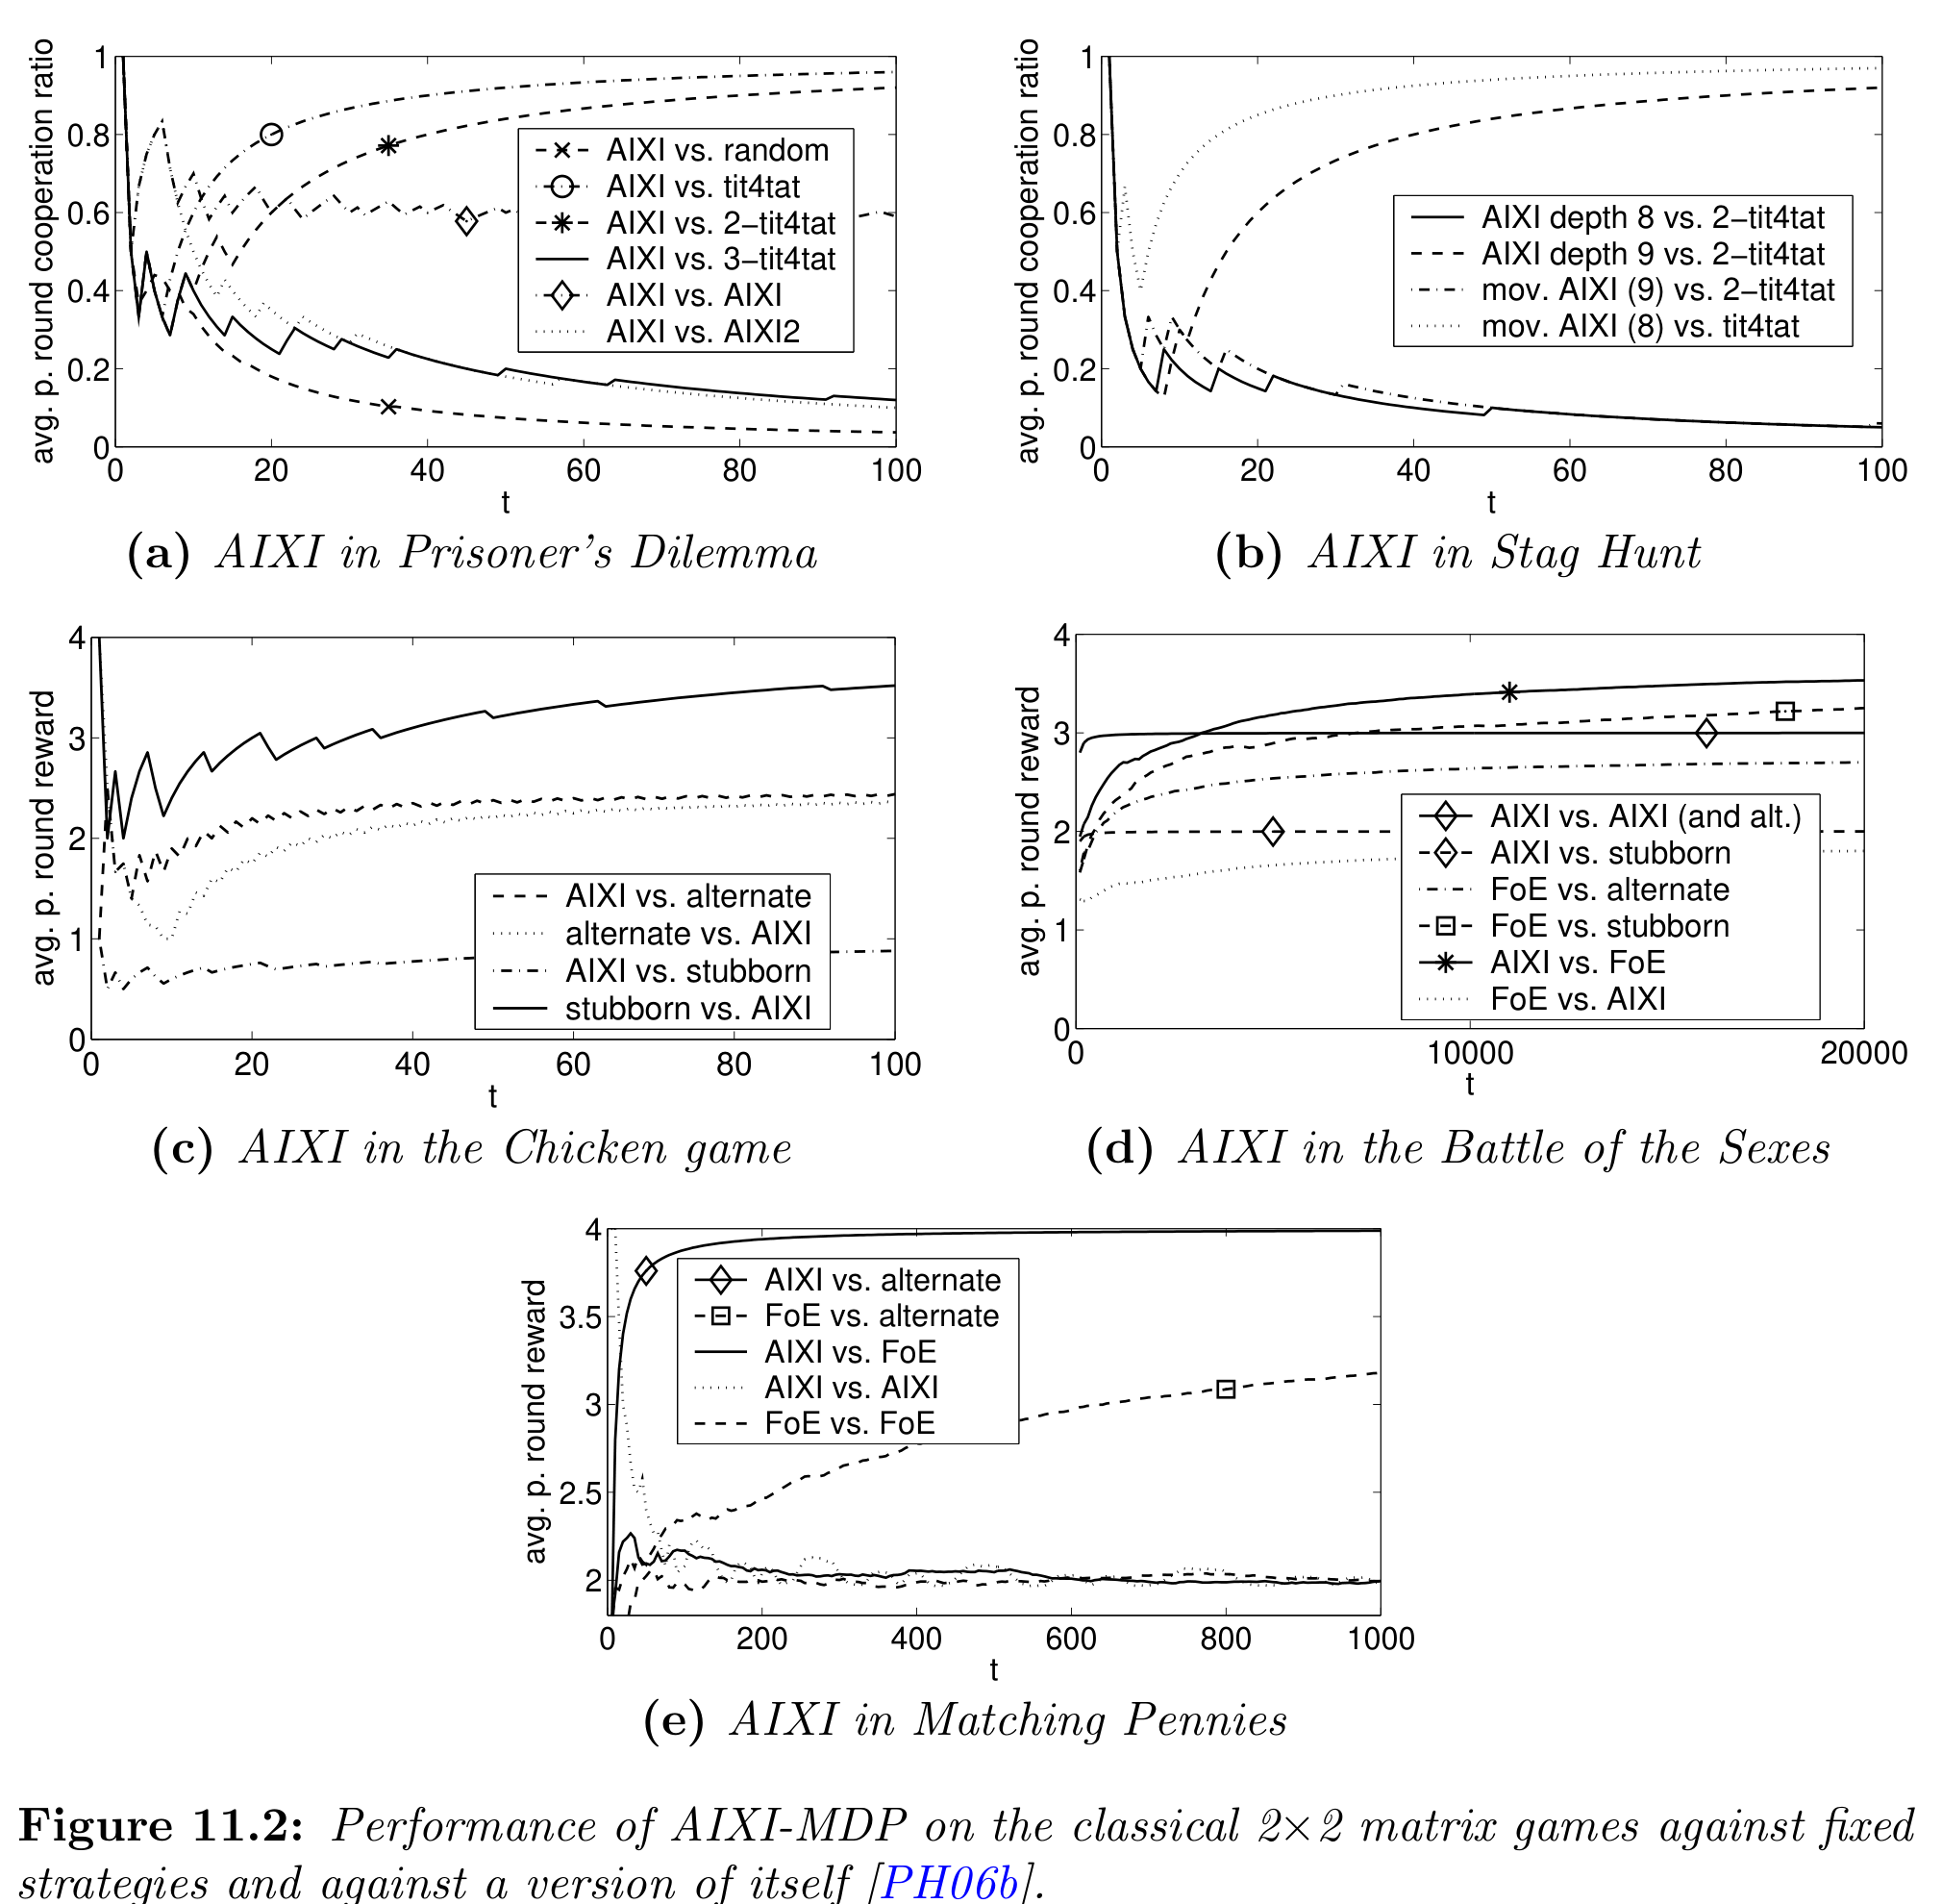
\includegraphics[height=0.88\textheight]{fig11_2_all}
  \end{center}
\end{frame}

% -----------------------------------------------------------------------------
\begin{frame}{Prisoner's Dilemma}
  \begin{columns}[T]
    \begin{column}{0.52\textwidth}
      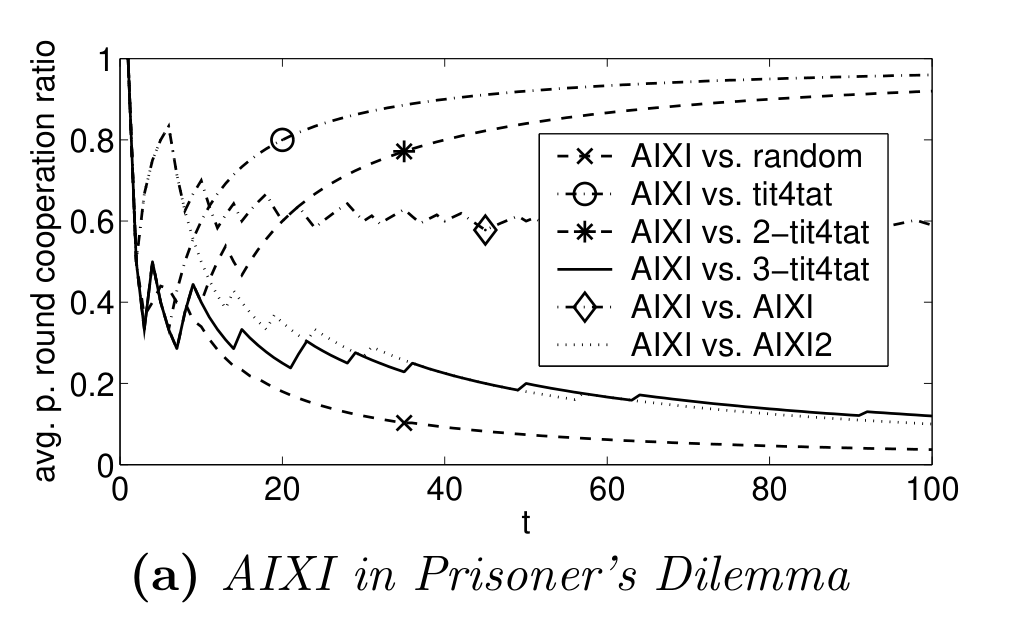
\includegraphics[width=\textwidth]{fig11_2a_pd}
    \end{column}
    \begin{column}{0.46\textwidth}
      {\small
      AIXI-MDP was compared to: \emph{random} (a coin flip each round),
      and \emph{$n$-tit-for-tat} for $n=1,2,3$ (cooperates first, then
      cooperates only if the opponent cooperated the last $n$ rounds in a
      row).

      \bigskip
      \textbf{Learns to cooperate} against \emph{1-tit-for-tat} and
      \emph{2-tit-for-tat}.

      \textbf{Learns to defect} against \emph{random} and
      \emph{3-tit-for-tat}.
      }
    \end{column}
  \end{columns}
  \explain{Why the split? \emph{1-tit-for-tat} is Markov (its next action
  depends only on the agent's single last action), so it genuinely lies in
  AIXI-MDP's model class $\Mmdp$, and the self-optimization guarantee
  (Theorem 7.3.6) can kick in. \emph{$n$-tit-for-tat} for $n\geq2$ is
  \textbf{not} Markov, yet AIXI-MDP still learns to cooperate against
  $2$-tit-for-tat, though not against the harder $3$-tit-for-tat -- it
  isn't given enough exploration to discover that deeper pattern. Against
  \emph{random}, defection is never punished, so always defecting really is
  reward-maximizing. Against a copy of \emph{itself}, symmetry makes both
  agents pick the same action every round; breaking that symmetry (e.g.\
  different horizons) instead made both agents believe the other would
  defect, spiraling into mutual defection.}
\end{frame}

% -----------------------------------------------------------------------------
\begin{frame}{Stag Hunt}
  \begin{columns}[T]
    \begin{column}{0.52\textwidth}
      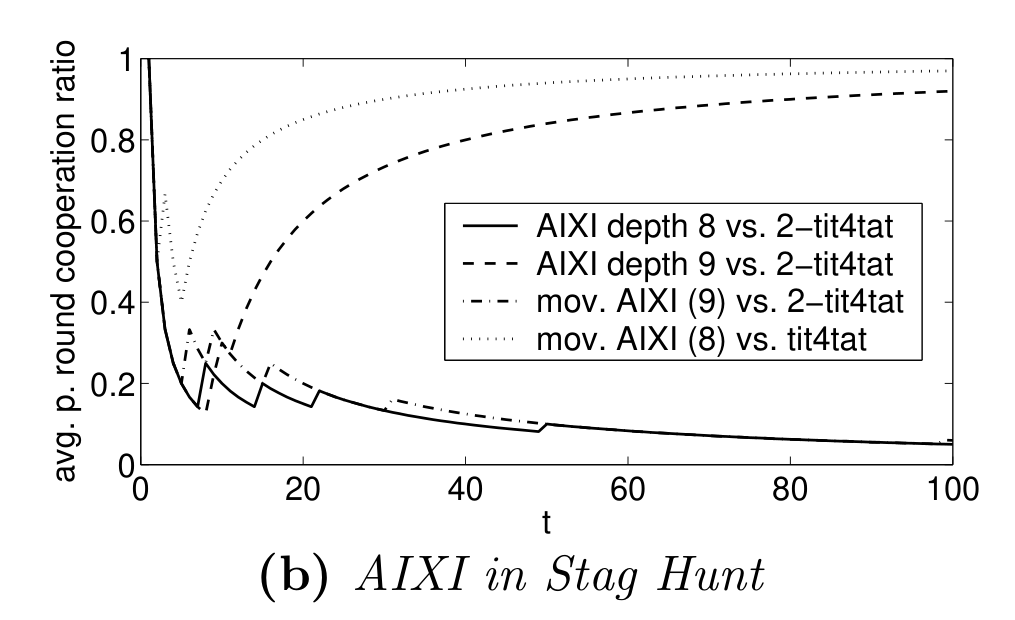
\includegraphics[width=\textwidth]{fig11_2b_staghunt}
    \end{column}
    \begin{column}{0.46\textwidth}
      {\small
      Stag Hunt resembles Prisoner's Dilemma, but mutual cooperation pays
      even \emph{more} than mutual defection. AIXI-MDP was tested against
      \emph{2-tit-for-tat}.

      \bigskip
      A \textbf{horizon-8} AIXI-MDP failed to learn to cooperate; a
      \textbf{horizon-9} AIXI-MDP succeeded (but still failed against the
      harder \emph{3-tit-for-tat}).
      }
    \end{column}
  \end{columns}
  \explain{One extra step of lookahead was enough to tip the balance from
  ``defect'' to ``cooperate'' here. Although an environment containing a
  \emph{2-tit-for-tat} opponent is not itself in the MDP model class
  $\Mmdp$, the mixture $\ximdp$ can still converge to behave like the true
  environment $\mu$ even when $\mu\notin\Mmdp$ (Corollary 3.4.2) -- model
  misspecification does not automatically doom the agent.}
\end{frame}

% -----------------------------------------------------------------------------
\begin{frame}{Chicken}
  \begin{columns}[T]
    \begin{column}{0.52\textwidth}
      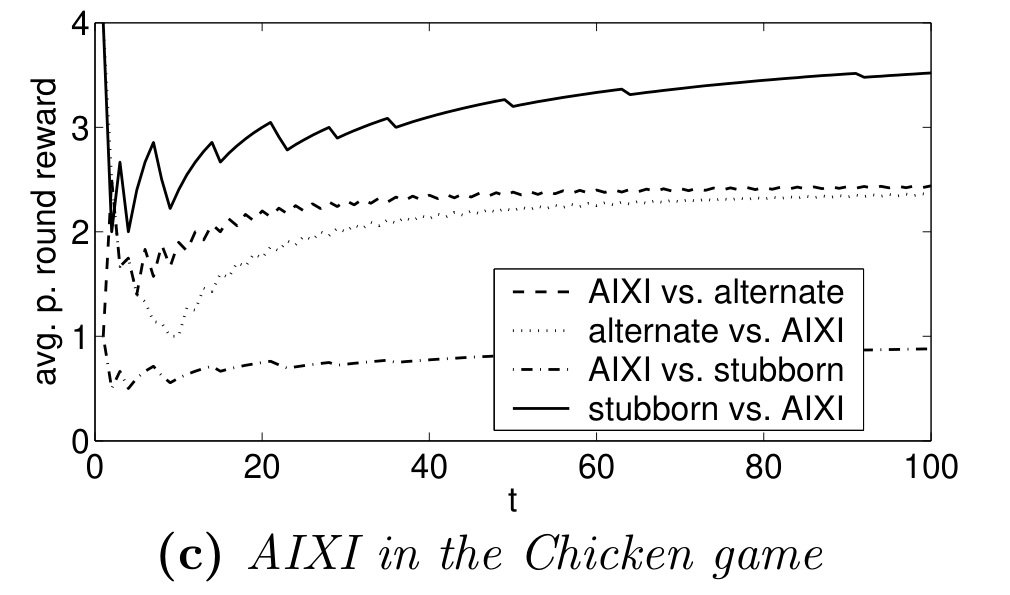
\includegraphics[width=\textwidth]{fig11_2c_chicken}
    \end{column}
    \begin{column}{0.46\textwidth}
      {\small
      In Chicken, the best strategy is to \emph{alternate} between going
      straight and swerving, letting the opponent swerve most of the time.
      Opponents tested: \emph{alternating} (alternates every round) and
      \emph{stubborn} (only swerves after the agent has gone straight
      \textbf{3} times in a row).
      }
    \end{column}
  \end{columns}
  \explain{AIXI-MDP quickly learns to go straight at the right moments
  against \emph{alternating}. Against \emph{stubborn}, however, it
  struggles to go straight three rounds in a row and so never discovers the
  optimal policy -- yet against a \emph{2-stubborn} variant (only requiring
  two straight-goes in a row) it \emph{does} learn the optimal sequence.
  This shows a real limitation: AIXI-MDP can fail to learn policies that
  require sustaining an unusual action for long enough to trigger a
  delayed payoff, when its lookahead is shorter than the required streak.
  When playing against itself, whichever copy has the \emph{higher}
  horizon learns to go straight more often, and ends up earning more
  reward overall.}
\end{frame}

% -----------------------------------------------------------------------------
\begin{frame}{Battle of the Sexes}
  \begin{columns}[T]
    \begin{column}{0.52\textwidth}
      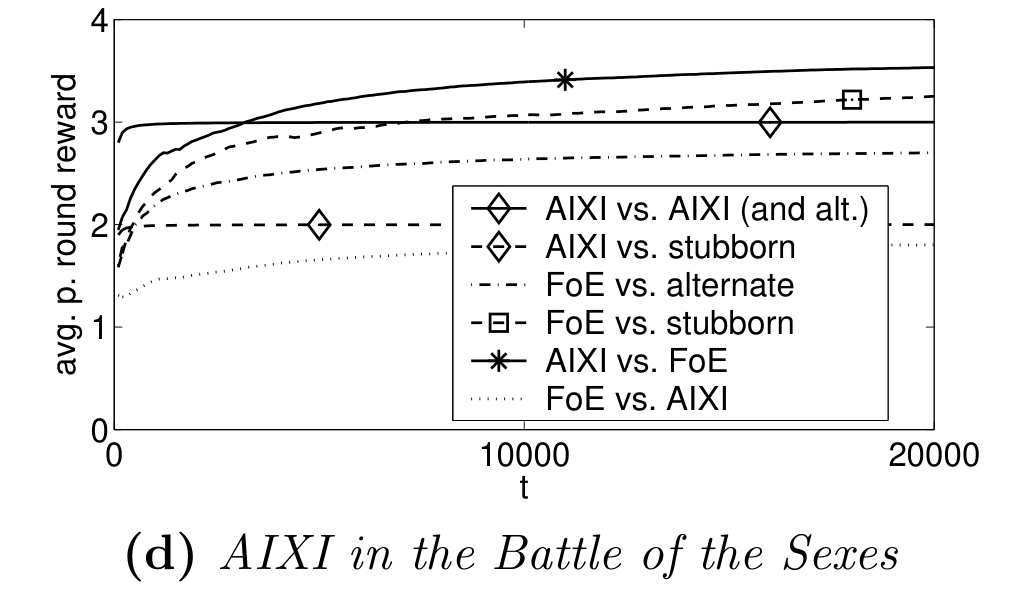
\includegraphics[width=\textwidth]{fig11_2d_bos}
    \end{column}
    \begin{column}{0.46\textwidth}
      {\small
      Both players want to take the \emph{same} action each round, and, to
      maximize joint reward, should also \emph{alternate} which action they
      coordinate on (so both players get a turn receiving the larger
      payoff). Opponents tested: \emph{alternating} and \emph{stubborn}.
      }
    \end{column}
  \end{columns}
  \explain{Against \emph{alternating}, AIXI-MDP learns to mirror the same
  alternation and achieves the socially optimal reward. Against
  \emph{stubborn}, it fails to learn the required alternating sequence and
  earns a below-average reward each round. When two AIXI-MDP copies play
  each other, \textbf{both} learn to alternate: each agent believes its
  opponent is Markov (depends only on the very last round), which makes
  ``alternate'' look like the right response to an opponent who alternates
  -- a mutually self-fulfilling prophecy, rather than deliberate
  coordination. Even so, both agents end up sharing the socially optimal
  average reward of $3$ each round.}
\end{frame}

% -----------------------------------------------------------------------------
\begin{frame}{Matching Pennies}
  \begin{columns}[T]
    \begin{column}{0.52\textwidth}
      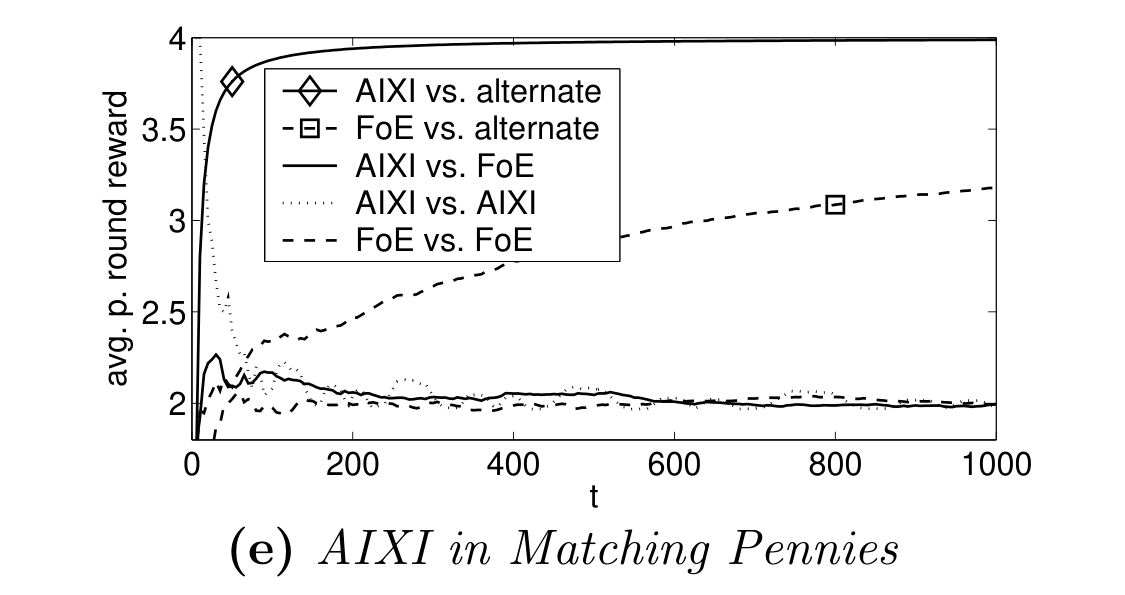
\includegraphics[width=\textwidth]{fig11_2e_mpennies}
    \end{column}
    \begin{column}{0.46\textwidth}
      {\small
      The only \textbf{zero-sum} game tested. The game-theoretic minimax
      strategy is to play each action with equal ($50/50$) probability.
      }
    \end{column}
  \end{columns}
  \explain{Against \emph{alternating}, AIXI-MDP learns the pattern and
  exploits it fully, achieving the maximum possible reward of $4$ every
  round -- far better than the cautious $50/50$ minimax strategy would give
  it, since the opponent here is exploitable. When two AIXI-MDP copies
  play each other with the \emph{same} horizon, the perfect symmetry of a
  zero-sum game locks them into always choosing the same (matching)
  action; as soon as that symmetry is broken (e.g.\ different horizons),
  both agents learn to alternate between their two actions instead.}
\end{frame}

% =============================================================================
\section{11.4 Exercises}
% =============================================================================

\begin{frame}{Exercises}
  Exercise numbers such as \texttt{[C25i]} are difficulty ratings (roughly,
  estimated hours of work; higher is harder), and a leading \texttt{C}
  marks an exercise that requires actual coding/implementation rather than
  pen-and-paper derivation.
  \begin{enumerate}
    \item \textbf{[C25i]} Implement AIXI-MDP in your chosen language and
      test it against the agents described in the experiments section
      (Section 11.3).
    \item \textbf{[C20]} Generalize AIXI-MDP to non-binary actions and
      observations, and test it on more complicated environments such as
      gridworlds.
    \item \textbf{[C20]} Determine the optimal agents for the given
      environment and opponents: tit-for-tat, stubborn, random, and
      alternating, etc.
    \item \textbf{[C23]} Given that AIXI-MDP assumes the environment is
      Markov, find a non-Markov agent which you expect AIXI-MDP to perform
      well against, and test it empirically.
  \end{enumerate}
\end{frame}

% =============================================================================
\section{11.5 History and References}
% =============================================================================

\begin{frame}{History and References}
  \begin{itemize}
    \item AIXI-MDP was first introduced in \textcolor{blue}{[PH06b]}, where
      it was compared against \textbf{Acting with Expert Advice}
      \textcolor{blue}{[PH05b]}, also called \textbf{Follow or Explore
      (FoE)} -- the \emph{active-learning} version of \emph{Prediction with
      Expert Advice} \textcolor{blue}{[HP04, HP05]}, which requires
      exploration. This extra exploration is achieved by forcing the FoE
      agent to explore with some exploration rate at every time step, a
      rate that decreases over time.
    \item The Bayesian approach (such as AIXI-MDP), expert-advice methods,
      and MDL-based (\emph{minimum description length}) methods were
      compared in the online-learning setting in \textcolor{blue}{[Pol06]}.
    \item The relationship between \emph{truncated} and \emph{untruncated}
      \emph{discounted} value functions -- relevant to the moving-horizon
      and time-inconsistency issues discussed above -- has been explored in
      \textcolor{blue}{[Hut06a, ASDH24]}.
  \end{itemize}
\end{frame}

% -----------------------------------------------------------------------------
\begin{frame}{Chapter Take-Aways}
  \begin{block}{Summary}
    \begin{itemize}
      \item AIXI-MDP is the first, simplest, and most tractable computable
        approximation of AIXI: restrict the model class to Markov Decision
        Processes, and the Bayes-optimal policy becomes brute-force
        computable via Algorithm 11.1.
      \item The Laplace estimator $\ximdp$ is a cheap, incremental,
        provably sound way to estimate MDP transition probabilities.
      \item The price of tractability is a restrictive assumption (Markov,
        no Grain of Truth): AIXI-MDP reliably learns against simple,
        Markov-compatible opponents, but can fail against opponents whose
        strategies require longer memory or longer sustained commitment
        than its lookahead allows.
    \end{itemize}
  \end{block}
\end{frame}

% =============================================================================
\end{document}
